\documentclass[8pt]{beamer}
%epackage[french]{babel}
\usepackage[latin1]{inputenc}
\usepackage{times}
\usepackage{wasysym}
\usepackage[T1]{fontenc}


\definecolor{mongris}{gray}{0.8}           % definition couleur grise
\newcommand{\dd}{\footnotesize $\Diamond$}

\newcommand{\HH}{ \vspace{0.5pt}\hrule}
\newcommand{\round}[1]{\lceil #1 \rfloor}  % notation arrondi
\def\eme{$^{\textrm{{\`e}me}}$}                  % i {\`e}me
\def\num{n^{\circ}}                        % numero
\def\Num{N^{\circ}}                        % Numero
\def\sinc{\mathrm{sinc}}                   % sinus cardinal
\def\ere{$^{\textrm{{\`e}re}}$}                % {\`e}re
\def\er{$^{\textrm{{e}r}}$}                % {\`e}re
\def\eg{\emph{e.g.} }                      % e.g.
\def\ie{\emph{i.e.} }                      % i.e.
\def\etc{\emph{etc.}}                       % etc
\def\cm{\,cm}                              % cm
\def\met{\,m}                              % m
\def\mm{\,mm}                              % mm
\def\deg{$^\circ$}                         % degres
\def\ud{\mathrm{d}}                        % pour dx dy ...


\def \R {{\Bbb R}}
\def \I {{\Bbb I}}
\def \H{{\Bbb H}}
\def \F {{\Bbb F}}
\def \S {{\Bbb S}}
\def \B {{\Bbb B}}
\def \Z {{\mathbb Z}}
\def \G {{\mathbb G}}
\def \L {{\mathcal{L}}}
\def \C {{\mathcal C}}
\def \P {{\mathcal P}}
\def \Q {{\mathcal Q}} 
\def \E{{\mathcal E}}
\def \D{{\mathcal D}}
\definecolor{mybluecolor}{RGB}{116,121,149}

\newcommand{\darky}[1]{{\usebeamercolor[fg]{block title example} #1}}
\newcommand{\myblue}[1]{{\color{mybluecolor}\aut{[#1]}}}

\newcommand{\ball}  {\ensuremath{B}}
\newcommand{\AMDR}{\operatorname{AMD}}
\newcommand{\AMD}{\operatorname{AMD}}

\newcommand{\MAset}{\ensuremath{\mathrm{A\!M}} }
\newcommand{\MAsetg}{\ensuremath{\MAset^g } }

\def \PS {{\aut{Planar-4-3-SAT}}}
\def \R {{\Bbb R}}
\def \I {{\Bbb I}}
\def \F {{\Bbb F}}
\def \S {{\Bbb S}}
\def \Z {{\mathbb Z}}
\def \L {{\mathcal{L}}}
\def \C {{\mathcal C}}
\def \P {{\mathcal P}}
\def \Q {{\mathcal Q}} 
\def \E{{\mathcal E}}
\def \D{{\mathcal D}}
\def \BD {{\bar{\mathcal{D}}}}
\def \etal {{\it et al.~}}
\def\arc{\mbox{arc}}
\definecolor{mongris}{gray}{0.8}          
\newcommand{\fup}[1]{\uparrow#1\uparrow}
\newcommand{\fdown}[1]{\downarrow#1\downarrow}
\newcommand{\sI}[1]{\overline{\tt #1}}
\newcommand{\iI}[1]{\underline{\tt #1}}
\newcommand{\e}[5]{#1 & #2 & #3 & #4 & #5 \\}
\newcommand{\eh}[5]{\text{#1} & \text{#2} &  \text{#3} &  \text{#4} & \text{#5}\\} 

\usepackage{beamerthemeliris2}
\useoutertheme{smoothbars}

\title[DGtal]{DGtal: Digital  Geometry Tools and Algorithms Library}
\subtitle{module G�om�trie 2D}

\author{}
%\author[DGtal~~~~~~~~~~~~~~~~~~~~~~~~~~David Coeurjolly]{David Coeurjolly}


 \newcommand{\fod}[2]{\multicolumn{2}{p{3.5cm}}{\emph{#1}\dotfill} &
      \multicolumn{2}{p{9cm}}{#2}\\}
    \newcommand{\fodt}[4]{\emph{#1} & {\footnotesize \textsl{#2}} & #3 & \small #4\\}
    % \newenvironment{ta}{\begin{tabular}{p{3.5cm}p{9cm}}}{\end{tabular}\\}
    \newenvironment{ta}{\begin{tabular}{crll}}{\end{tabular}\\}
    % \vfill


\newcommand{\aut}[1]{{\sc #1}}             % auteur en small capsu


%\institute%[XXX]
%{%
%
%  {\bf Laboratoire d'InfoRmatique en Image et Syst�mes d'information} \\
%  { \scriptsize{
%  LIRIS UMR 5205 CNRS/INSA de Lyon/Universit� Claude Bernard Lyon 1/Universit� Lumi�%re Lyon 2/Ecole Centrale de Lyon\\
%  INSA de Lyon, b�timent J. Verne\\
%  20, Avenue Albert Einstein - 69622 Villeurbanne cedex\\
%  \url{http://liris.cnrs.fr}}
%  }
%}



\graphicspath{{./Images/}}


\begin{document}

\small








\begin{frame}[plain]
  \titlepage
\end{frame}



%\begin{frame}
%  \frametitle{Table of Contents}
%  \tableofcontents
%\end{frame}


\section{Objectifs}

\begin{frame}
\frametitle{Objectives}

Tools that help in analysing any one-dimensional discrete structures in a generic framework. 

  \begin{block}{Examples in digital geometry}
    \begin{itemize}
    \item digital curves
      \begin{itemize}
      \item 2d, 3d, nd
      \item 4-connected, 8-connected, disconnected
      \item pixels, interpixels, points
      \item open or closed
      \end{itemize}
		\item chain codes
    \end{itemize}
  \end{block}

\alert{Constant structures, not mutable} 

\end{frame}






\section{Exemple}



\begin{frame}
  \frametitle{Exemple (greedy-dss-decomposition.cpp) }
http://liris.cnrs.fr/dgtal/doc/nightly/
 \begin{center}
   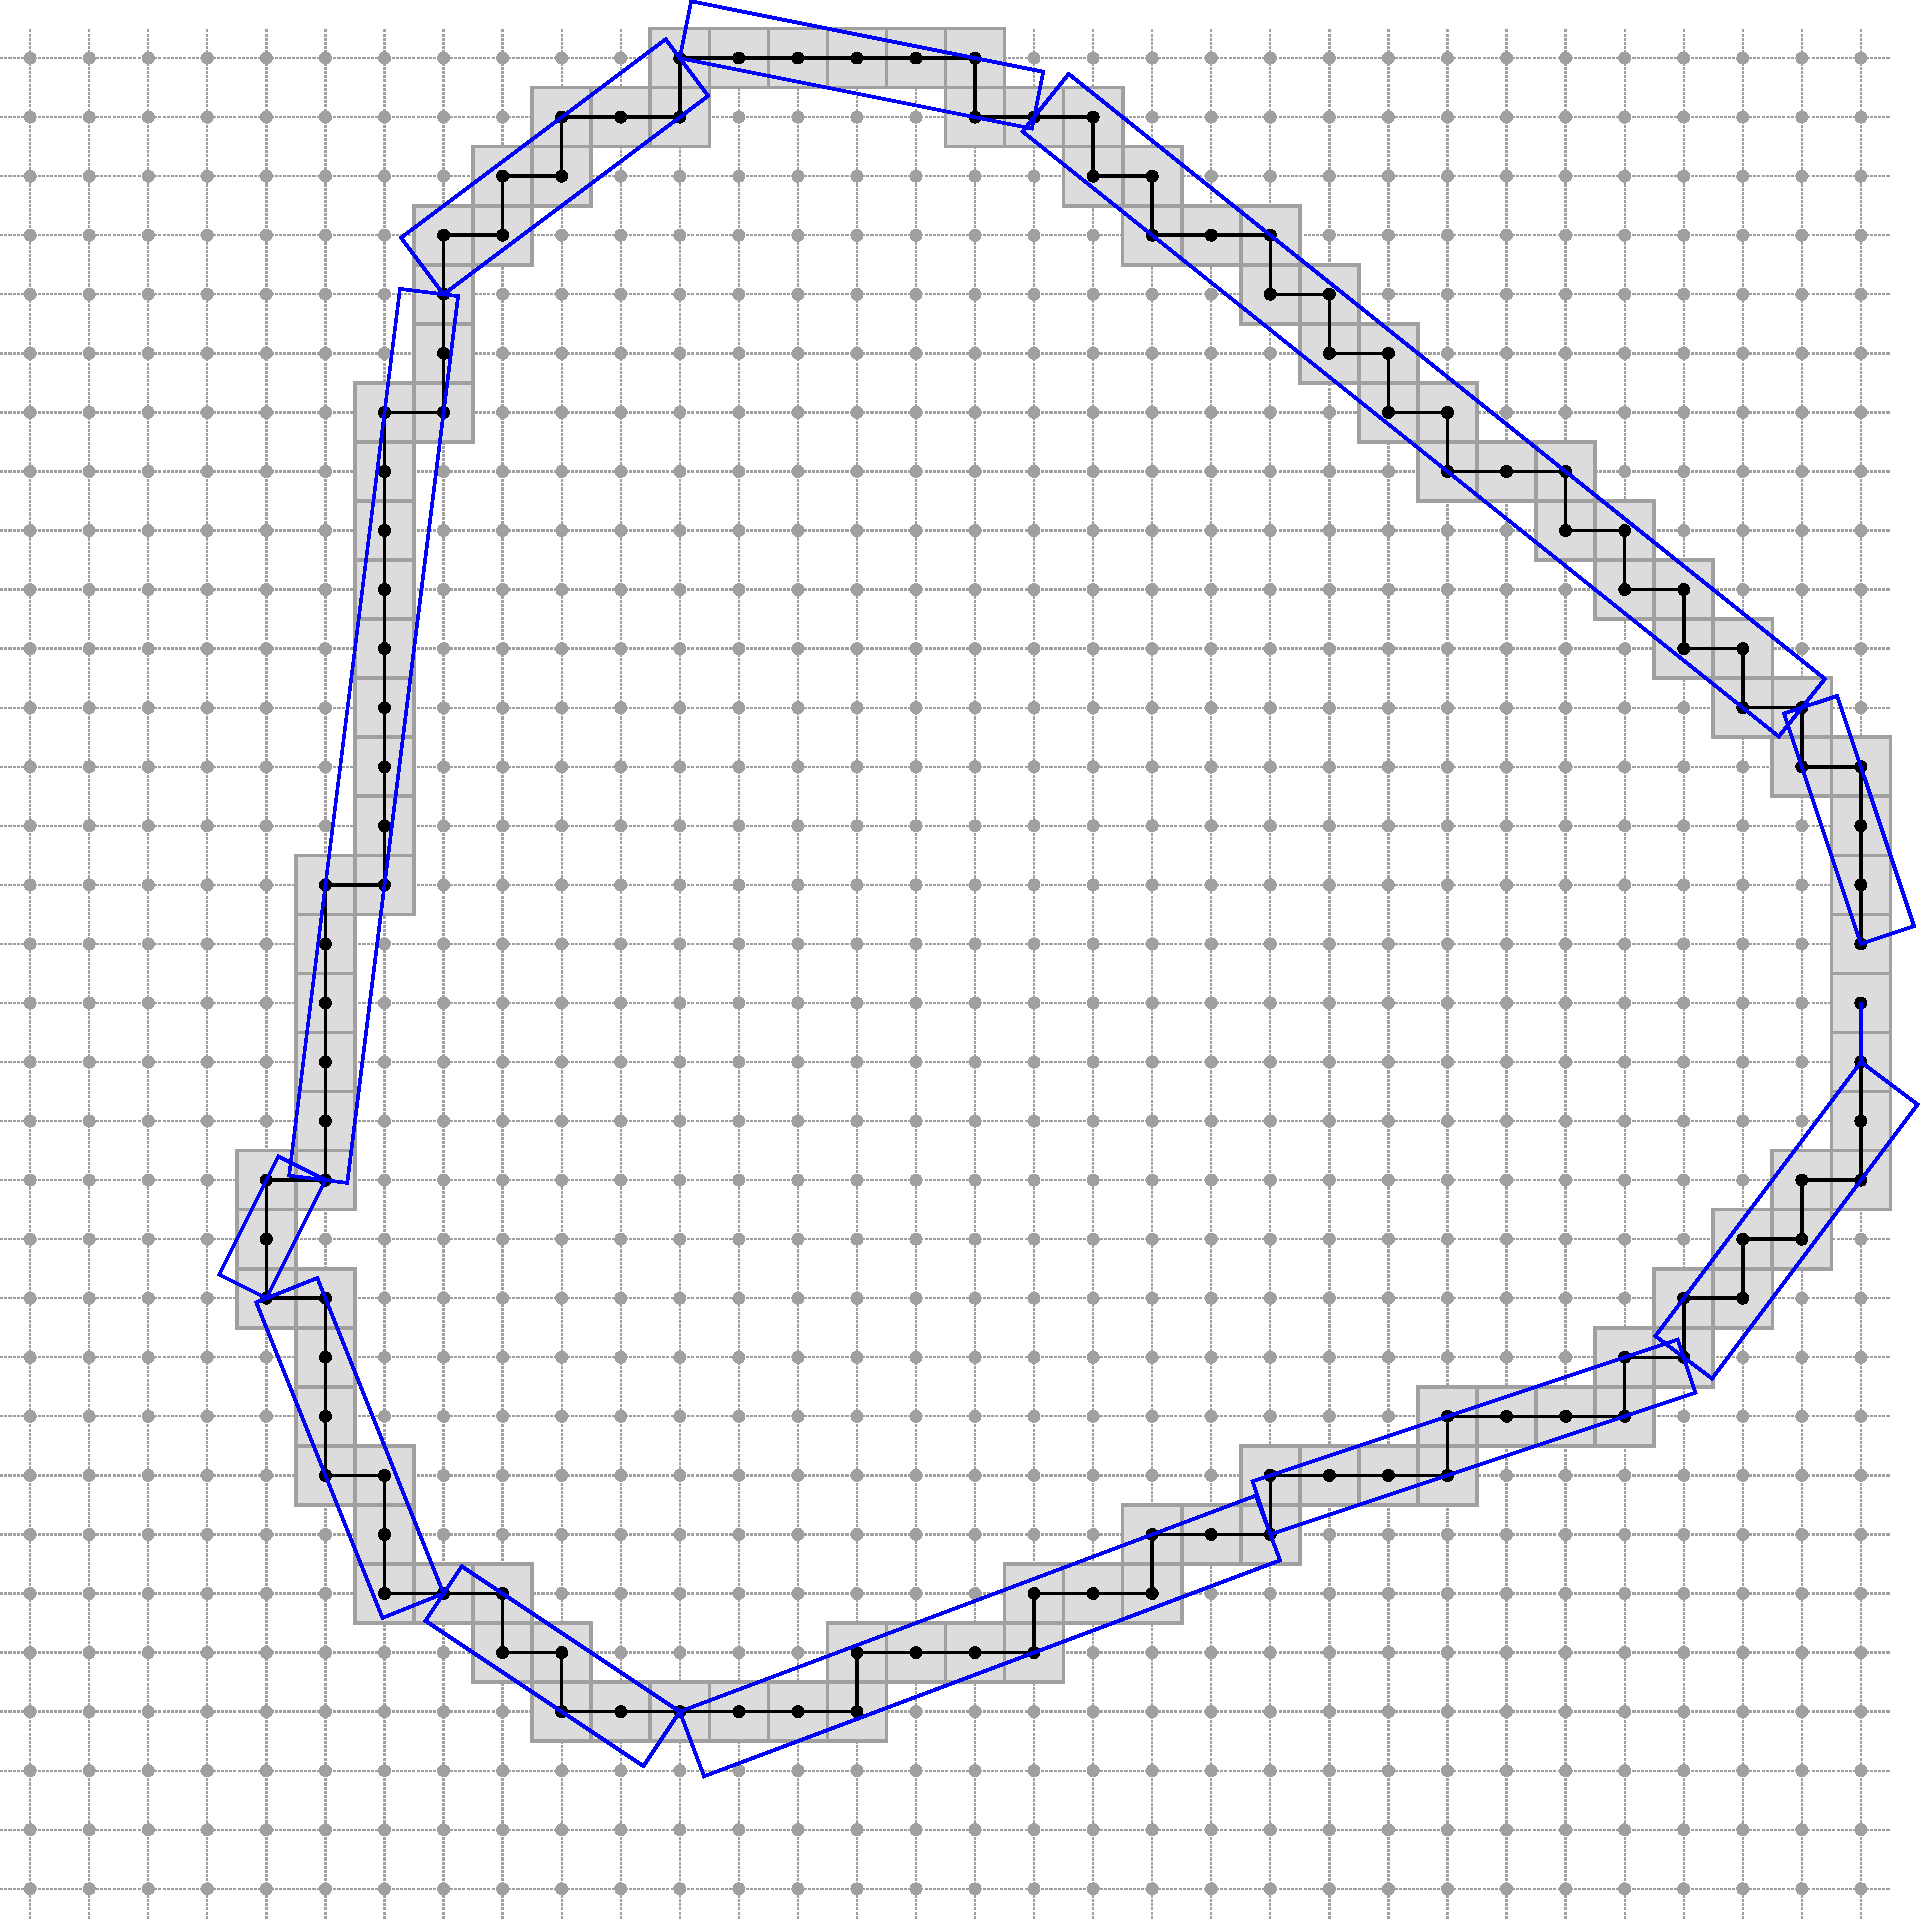
\includegraphics[width=1\textwidth]{segmentation}
 \end{center}
\end{frame}


\begin{frame}
  \frametitle{Code}
 \begin{center}
	\only<1>{
greedy-dss-decomposition.cpp
   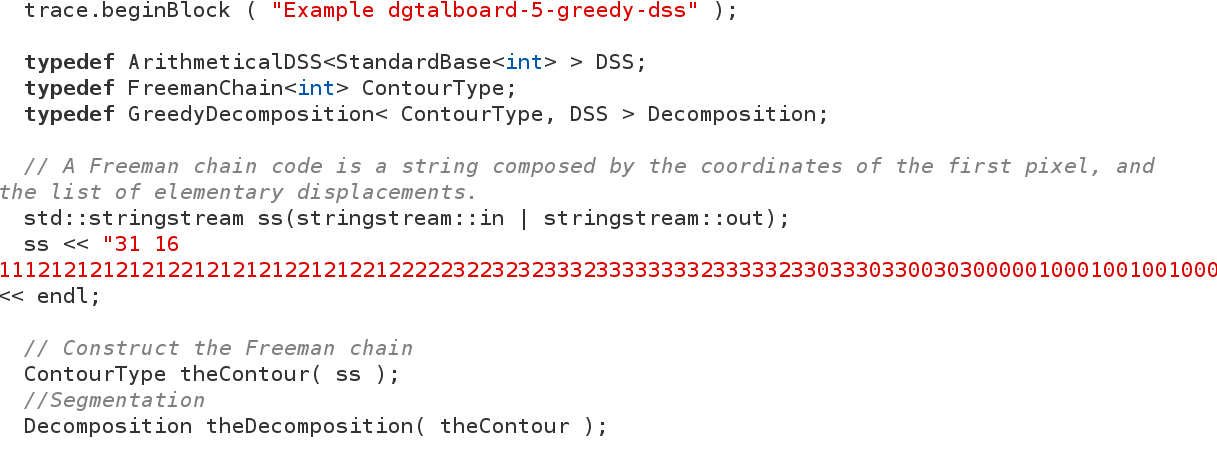
\includegraphics[width=1\textwidth]{code1.png}
	}
	\only<2>{
greedy-dss-decomposition.cpp
   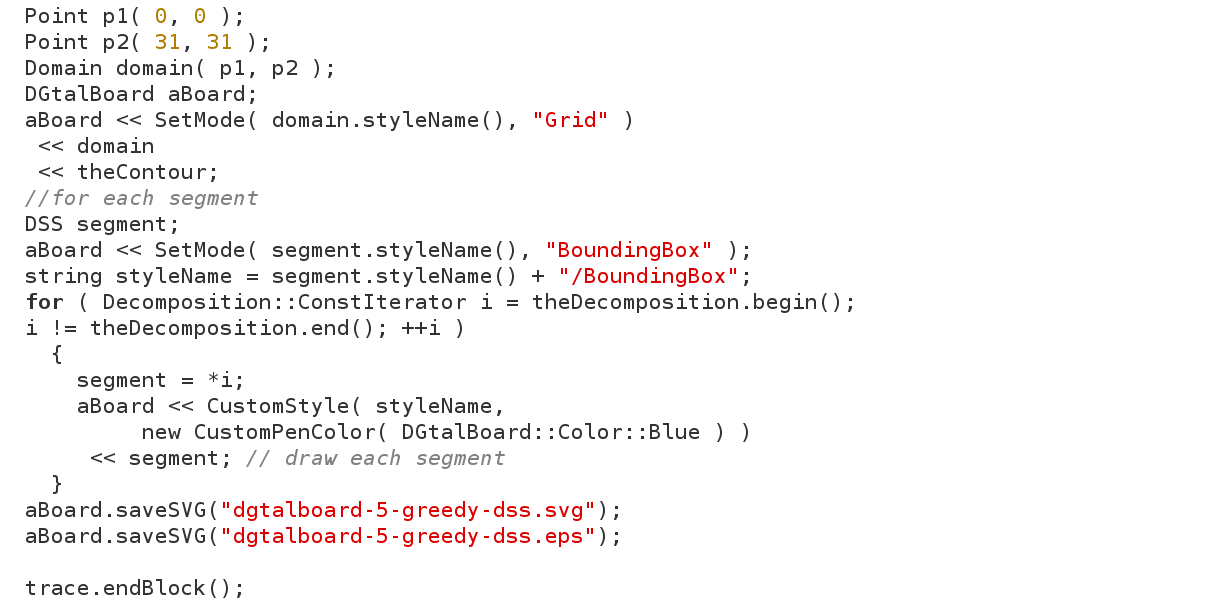
\includegraphics[width=1\textwidth]{code2.png}
	}
	\only<3>{
GreedyDecomposition.ih
   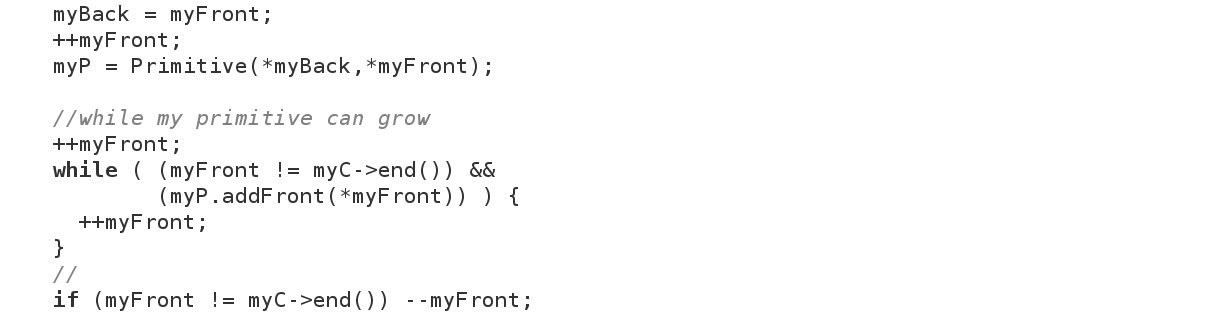
\includegraphics[width=1\textwidth]{code3.png}
	}
	\only<4>{
ArithmeticalDSS.ih
   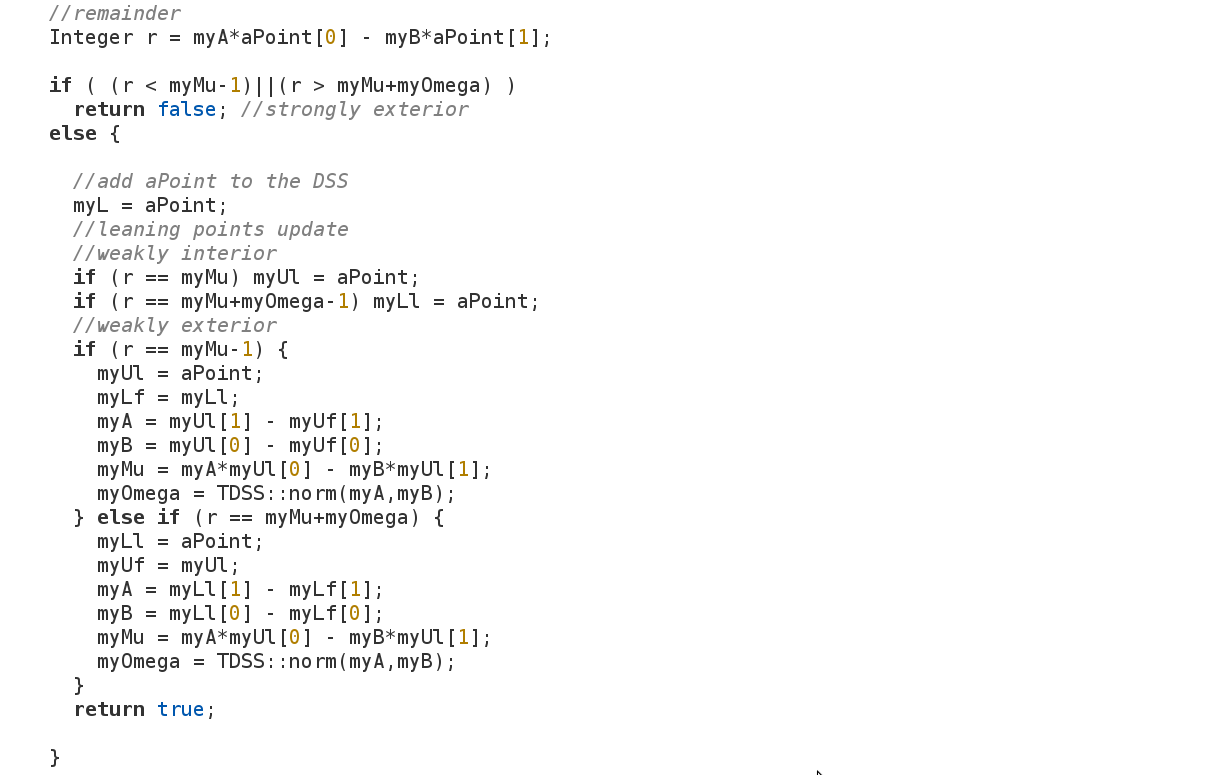
\includegraphics[width=1\textwidth]{code4.png}
	}

 \end{center}
\end{frame}



\section{Choix}


\begin{frame}
  \frametitle{Choix algorithmiques}

  \begin{block}{Algorithme de Debled et Reveill�s (1995)}
    \begin{itemize}
    \item caract�ristiques $a$, $b$, $\mu$, $\omega$
    \item 4 points d'appui
		\item premier et dernier points
    \item pas de changement d'octant, mais une orientation
    \end{itemize}
  \end{block}

  \begin{exampleblock}{~~~~~~~~~~~~(2,5,0,7)
~~~~~~~~~~~~~~~~~~~~~~~~~~~~~~~~~~~~~~~~~~~~~~~~~~~~~~~~~ (-2,-5,-6,7)}
 \begin{center}
   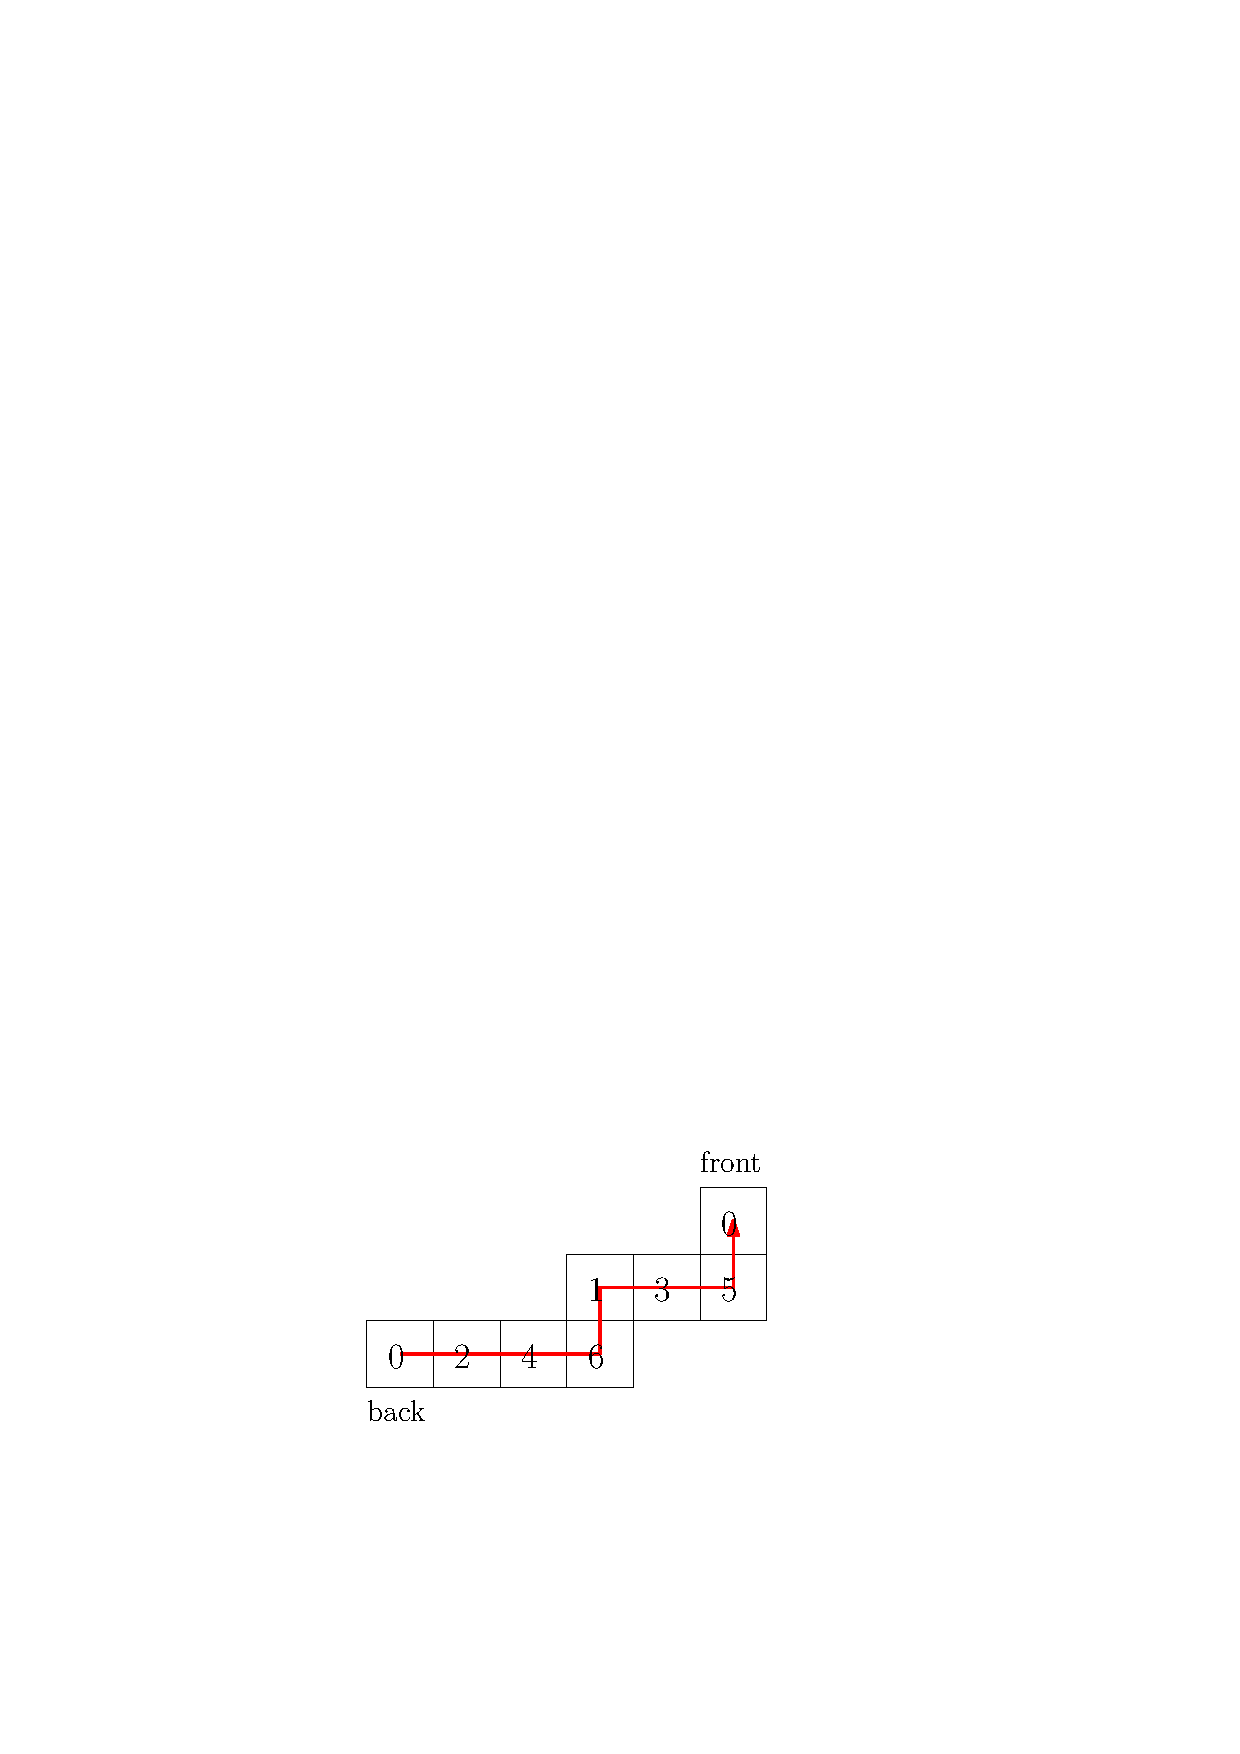
\includegraphics[width=0.3\textwidth,page=1]{DSS}\hspace{0.2\textwidth}
   \includegraphics[width=0.3\textwidth,page=2]{DSS}
 \end{center}
  \end{exampleblock}

\end{frame}

\begin{frame}
  \frametitle{Choix d'impl�mentation}
  

  \begin{block}{Param�tres templates}
    \begin{itemize}
    \item Entier (Domaine ?)
%pas de domaine (image)
    \item Connexit� $\{ \text{na�f}, \text{standard} \}$ 
%eviter les redondances entre les versions
    \end{itemize}
  \end{block}

  \begin{block}{M�thodes principales}
    \begin{itemize}
    \item Initialisation � partir de deux points (un seul point ?)
    \item ajout d'un point � l'avant
		  \begin{itemize}
		  \item \emph{addFront}
			\item prends un point comme param�tre en entr�e (un vecteur, un caract�re ?)
		  \item retourne un booleen (V si DSS, F sinon)
		  \end{itemize}
    \item retrait d'un point � l'arri�re
		  \begin{itemize}
		  \item \emph{removeBack}
			\item pas de param�tre en entr�e
		  \item retourne un booleen (V s'il reste plus de 2 points, F sinon)
		  \end{itemize}
    \end{itemize}
  \end{block}


\end{frame}



\section{Bilan et perspectives}

\begin{frame}
  \frametitle{Bilan}
 

 \begin{block}{D�finition des concepts (� discuter) } 
   \begin{itemize}
   \item courbe : liste (circulaire) de points (ordre)
		\begin{itemize}
			\item fournit un it�rateur sur les points (ou les vecteurs de d�placement entre deux points cons�cutifs ?)
		\end{itemize}
   \item primitive : courbe v�rifiant une propri�t� donn�e
		 \begin{itemize}
		 \item initialisation (un point plut�t que deux pour que la propri�t� soit toujours v�rifi�e) 
		 \item ajout � l'avant (un point, un vecteur d�placement ?), retourne V si la propri�t� reste vraie (et le point est ajout�), F sinon (et le point n'est pas ajout� pour que la propri�t� reste vraie) 
		 \item ...
%\only<1>{
%		 \item ...
%}
%\only<2>{
%		 \item retrait � l'arri�re s'il y a plus d'un point, la propri�t� reste toujours vraie
%}
		 \end{itemize}
   \item d�composition : liste (circulaire) de primitives recouvrant une courbe (ordre)
		\begin{itemize}
			\item fournit un it�rateur sur les primitives
%			\item mod�lise les relations entre les points de la courbe et les primitives ? 
		\end{itemize}
   \end{itemize}
 \end{block}


\end{frame}

\begin{frame}
  \frametitle{Perspectives}

 \begin{block}{Regarder ce qu'on a fait} 
   \begin{itemize}
   \item Am�liorations de \emph{FreemanChain}, \emph{ArithmeticalDSS}, \emph{GreedySegmentation} (si besoin)
   \item Ecriture des concepts de courbe, primitive et d�composition (si on est d'accord).        
   \end{itemize}
 \end{block}

 \begin{block}{Aller plus loin...} 
   \begin{itemize}
   \item D'autres courbes (8-connexes ?)
		 \begin{itemize}
		 \item discr�tisation de courbes euclidiennes
		 \item extraction du bord de r�gions connexes
		 \end{itemize}
   \item D'autres primitives (il y a le choix!)
   \item D'autres d�compositions (couverture)        
   \end{itemize}

 \end{block}

\end{frame}






\end{document}



